
%%--------------------------------------------------
%% CPO: Selected Responce Questions
%%--------------------------------------------------


%% Chapter 2: The Laws of Motion
%%--------------------------------------------------


%% Learning Objectives
%%--------------------------------------------------

%% Recognize that force is needed to change an object’s motion. 
%% Explain Newton’s first law. 
%% Describe how inertia and mass are related.
%% Define and calculate acceleration. 
%% Explain the relationship between force, mass, and acceleration. 
%% Determine mass, acceleration, or force given two of the quantities. 
%% Describe the motion of an object in free fall. 
%% Calculate speed and distance for an object in freefall.
%% Distinguish between mass and weight. 
%% Explain how air resistance affects the motion of objects. 
%% Describe motion using graphs. 
%% Use a position versus time graph to calculate speed from the slope. 
%% Use a speed versus time graph to calculate acceleration and distance.


%% CPO Multiple Choice Questions
%%--------------------------------------------------
\element{cpo-mc}{
\begin{question}{cpo-ch02-q01}
    The inertia of an object is related to its:
    \begin{multicols}{2}
    \begin{choices}
        \wrongchoice{mass and speed.}
        \wrongchoice{mass and force.}
      \correctchoice{mass only.}
        \wrongchoice{speed only.}
    \end{choices}
    \end{multicols}
\end{question}
}

\element{cpo-mc}{
\begin{question}{cpo-ch02-q02}
    Newton's first law is also known as the law of:
    \begin{multicols}{2}
    \begin{choices}
      \correctchoice{inertia.}
        \wrongchoice{universal gravitation.}
        \wrongchoice{force pairs.}
        \wrongchoice{unbalanced forces.}
    \end{choices}
    \end{multicols}
\end{question}
}

\element{cpo-mc}{
\begin{question}{cpo-ch02-q03}
    If the net force acting on a moving object is zero,
        the object will:
    \begin{choices}
        \wrongchoice{slow down and, eventually, stop.}
        \wrongchoice{continue at the same speed but change direction.}
        \wrongchoice{continue in the same direction but change speed.}
      \correctchoice{continue in the same direction with no change in speed.}
    \end{choices}
\end{question}
}

\element{cpo-mc}{
\begin{question}{cpo-ch02-q04}
    A ball with mass of \SI{1}{\kilo\gram} is moving in a straight line at the same speed as a ball with mass of \SI{10}{\kilo\gram}.
    Both balls are brought to rest in \SI{4}{\second}.
    What is true of the force required to stop the balls?
    \begin{choices}
      \correctchoice{It takes less force to stop the \SI{1}{\kilo\gram} ball because it has less inertia.}
        \wrongchoice{It takes more force to stop the \SI{1}{\kilo\gram} ball because it has more inertia.}
        \wrongchoice{It takes the same force to stop both balls because they are moving at the same speed.}
        \wrongchoice{It takes less force to stop the \SI{10}{\kilo\gram} ball because it has less inertia.}
    \end{choices}
\end{question}
}

\element{cpo-mc}{
\begin{question}{cpo-ch02-q05}
    If an object is accelerated, all of the following may occur \emph{except}:
    \begin{choices}
        \wrongchoice{a change in speed.}
        \wrongchoice{a change of direction.}
      \correctchoice{it remains motionless.}
        \wrongchoice{a change of direction and speed.}
    \end{choices}
\end{question}
}

\element{cpo-mc}{
\begin{question}{cpo-ch02-q06}
    The newton is defined as the:
    \begin{choices}
        \wrongchoice{force of gravity acting on a one kilogram object at Earth's surface.}
      \correctchoice{force that can give a \SI{1}{\kilo\gram} mass an acceleration of \SI{1}{\meter\per\second\squared}.}
        \wrongchoice{speed of an object when under the influence of Earth's gravitational field.}
        \wrongchoice{mass of an object that is accelerated at a rate of \SI{1}{\meter\per\second\squared}.}
    \end{choices}
\end{question}
}

\element{cpo-mc}{
\begin{question}{cpo-ch02-q07}
    All of the following examples of motion can be caused by a force \emph{except} a:
    \begin{choices}
        \wrongchoice{car moving around a corner at \SI{30}{\mile\per\hour}.}
      \correctchoice{boat speeding down a lake at \SI{100}{\kilo\meter\per\hour}.}
        \wrongchoice{skateboarder rolling to a stop.}
        \wrongchoice{motorcycle accelerating from \SIrange{0}{70}{\mile\per\hour} in \SI{4.2}{\second}.}
    \end{choices}
\end{question}
}

\element{cpo-mc}{
\begin{question}{cpo-ch02-q08}
    The equation that correctly expresses Newton's second law is:
    \begin{choices}
        %\wrongchoice{$force=mass \div\ acceleration$.}
        \wrongchoice{$force=mass / acceleration$.}
      \correctchoice{$force=mass \times\ acceleration$.}
        \wrongchoice{$force=mass + acceleration$.}
        \wrongchoice{$force=mass - acceleration$.}
    \end{choices}
\end{question}
}

\element{cpo-mc}{
\begin{question}{cpo-ch02-q09}
    The term that best describes the motion of an object that is slowing down is:
    \begin{multicols}{2}
    \begin{choices}
        \wrongchoice{free fall.}
        \wrongchoice{gravity.}
      \correctchoice{deceleration.}
        \wrongchoice{uniform.}
    \end{choices}
    \end{multicols}
\end{question}
}

\element{cpo-mc}{
\begin{question}{cpo-ch02-q10}
    Units of measurement used to label a quantity of acceleration are:
    \begin{multicols}{2}
    \begin{choices}
        \wrongchoice{\si{\centi\meter\squared\per\second}}
        \wrongchoice{\si{\second\squared\per\centi\meter}}
        \wrongchoice{\si{\centi\meter\per\second}}
      \correctchoice{\si{\centi\meter\per\second\squared}}
    \end{choices}
    \end{multicols}
\end{question}
}

\element{cpo-mc}{
\begin{question}{cpo-ch02-q11}
    The rate of change in the speed of an object is known as:
    \begin{multicols}{2}
    \begin{choices}
        \wrongchoice{velocity.}
        \wrongchoice{displacement.}
      \correctchoice{acceleration.}
        \wrongchoice{equilibrium.}
    \end{choices}
    \end{multicols}
\end{question}
}

\element{cpo-mc}{
\begin{question}{cpo-ch02-q12}
    Acceleration of an object \emph{must} be caused by a force that is:
    \begin{multicols}{2}
    \begin{choices}
        \wrongchoice{positive.}
        \wrongchoice{zero.}
        \wrongchoice{negative.}
      \correctchoice{not zero.}
    \end{choices}
    \end{multicols}
\end{question}
}

\element{cpo-mc}{
\begin{question}{cpo-ch02-q13}
    The metric unit of force preferred by scientists is the:
    \begin{multicols}{2}
    \begin{choices}
        \wrongchoice{kilogram (\si{\kilo\gram})}
      \correctchoice{newton (\si{\newton})}
        \wrongchoice{mina (mna)}
        \wrongchoice{pound (\si{\pound})}
    \end{choices}
    \end{multicols}
\end{question}
}

\element{cpo-mc}{
\begin{question}{cpo-ch02-q14}
    Toby glances at the speedometer on his bicycle as he begins to roll downhill.
    It indicates he is traveling at \SI{12}{\mile\per\hour} when he initially looks at it and \SI{20}{\mile\per\hour} \SI{4}{\second} later.
    His acceleration is:
    \begin{multicols}{2}
    \begin{choices}
      \correctchoice{\SI{2}{\mile\per\hour\per\second}}
        \wrongchoice{\SI{3}{\mile\per\hour\per\second}}
        \wrongchoice{\SI{5}{\mile\per\hour\per\second}}
        \wrongchoice{\SI{8}{\mile\per\hour\per\second}}
    \end{choices}
    \end{multicols}
\end{question}
}

\element{cpo-mc}{
\begin{question}{cpo-ch02-q15}
    The inertia of two objects \emph{must} be the same if:
    \begin{choices}
        \wrongchoice{The acceleration of both object is the same.}
      \correctchoice{The same force causes the same acceleration in both objects.}
        \wrongchoice{The product of their mass and speed are the same.}
        \wrongchoice{Both objects are moving at the same speed in the same direction.}
    \end{choices}
\end{question}
}

\element{cpo-mc}{
\begin{question}{cpo-ch02-q16}
    A ball with a mass of \SI{1}{\kilogram} is moving in a straight line at the same speed as a ball with a mass of \SI{10}{\kilo\gram}.
    What \emph{must} be true of the force required to stop the balls?
    \begin{choices}
        \wrongchoice{It takes the same force to stop both balls because they are moving at the same speed.}
        \wrongchoice{It takes more force to stop the \SI{10}{\kilo\gram} ball because is has more inertia.}
        \wrongchoice{It takes more force to stop the \SI{1}{\kilo\gram} ball because it has more inertia.}
      \correctchoice{The forces required to stop the balls cannot be determined from the information given.}
    \end{choices}
\end{question}
}

\element{cpo-mc}{
\begin{question}{cpo-ch02-q17}
    Two forces are applied to a \SI{2.0}{\kilo\gram} block on a frictionless,
        horizontal surface, as shown in the following diagram:
    \begin{center}
    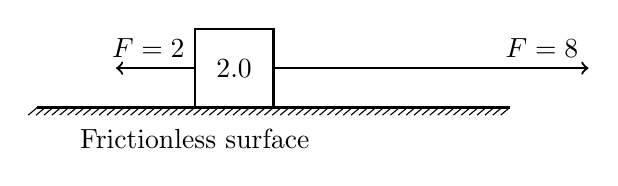
\begin{tikzpicture}
        %% Force
        \draw[thick,<-] (-1.0,0.5) -- (-0.0,0.5)
            node[above left] {$F=\SI{2}{\newton}$};
        \draw[thick,->] (1.0,0.5) -- (5.0,0.5)
            node[above left] {$F=\SI{8}{\newton}$};
        %% Block
        \draw[thick] (0,0) rectangle (1,1);
        \node[anchor=center] at (0.5,0.5) {\SI{2.0}{\kilo\gram}};
        %% Floor
        \draw[thick] (-2,0) -- (4,0);
        \foreach \x in {-20,-19,...,40}
            \draw[thin] (\x mm,0cm) -- ++ (220:0.15cm);
        \node[anchor=north] at (0,-0.15) {Frictionless surface};
    \end{tikzpicture}
    \end{center}
    The acceleration of the block is:
    \begin{multicols}{2}
    \begin{choices}
      \correctchoice{\SI{3.0}{\meter\per\second\squared} to the right.}
        \wrongchoice{\SI{3.0}{\meter\per\second\squared} to the left.}
        \wrongchoice{\SI{5.0}{\meter\per\second\squared} to the right.}
        \wrongchoice{\SI{5.0}{\meter\per\second\squared} to the left.}
    \end{choices}
    \end{multicols}
\end{question}
}

\element{cpo-mc}{
\begin{question}{cpo-ch02-q18}
    A series of forces was applied to each of two blocks, $A$ and $B$.
    The graphs below show the relationship between the force and the acceleration for each block.
    \begin{center}
    \begin{tikzpicture}
        \begin{axis}[
            axis y line=left,
            axis x line=bottom,
            axis line style={->},
            ylabel={force},
            y unit=\si{\newton},
            ytick={0,1,2,3,4},
            ymin=0,ymax=4,
            xlabel={Acceleration},
            x unit=\si{\meter\per\second\squared},
            xtick={0,1,2,3,4},
            xmin=0,xmax=4,
            grid=major,
            width=0.8\columnwidth,
            height=0.5\columnwidth,
            very thin,
        ]
        %% Block A
        \addplot[black,line width=1pt,domain=1:3]{x}
            node[anchor=north west,pos=1.0] {$A$};
        \addplot coordinates {(1,1) (2,2) (3,3)};
        %% Block B
        \addplot[black,line width=1pt,domain=1:1.5]{2*x}
            node[anchor=south,pos=1.0] {$B$};
        \addplot coordinates {(0.5,1) (1,2) (1.5,3)};
        \end{axis}
    \end{tikzpicture}
    \end{center}
    Compared to the mass of block $A$, the mass of block $B$ is:
    \begin{multicols}{2}
    \begin{choices}
        \wrongchoice{the same.}
        \wrongchoice{twice as great.}
      \correctchoice{half as great.}
        \wrongchoice{four times as great.}
    \end{choices}
    \end{multicols}
\end{question}
}

\element{cpo-mc}{
\begin{question}{cpo-ch02-q19}
    When an object is accelerating due to the force of gravity with no other forces acting on it, it is:
    \begin{multicols}{2}
    \begin{choices}
        \wrongchoice{changing directions.}
        \wrongchoice{motionless.}
      \correctchoice{in free fall.}
        \wrongchoice{at terminal speed.}
    \end{choices}
    \end{multicols}
\end{question}
}

%% NOTE: Rethink this question
%\element{cpo-mc}{
%\begin{questionmult}{cpo-ch02-Q20}
%    The acceleration due to gravity is:
%    \begin{choices}
%      \correctchoice{\SI{9.8}{\meter\per\second\squared}.}
%      \correctchoice{signified by the letter $g$.}
%      \correctchoice{a downward acceleration.}
%    \end{choices}
%\end{questionmult}
%}

\element{cpo-mc}{
\begin{question}{cpo-ch02-q21}
    When you throw a ball up in the air, it travels up and then stops instantaneously before falling back down.
    At the point where it stops and changes direction to fall back down its:
    \begin{multicols}{2}
    \begin{choices}
        \wrongchoice{acceleration is zero.}
      \correctchoice{velocity is zero.}
        \wrongchoice{force is zero.}
        \wrongchoice{mass is zero.}
    \end{choices}
    \end{multicols}
\end{question}
}

\element{cpo-mc}{
\begin{question}{cpo-ch02-q22}
    A bungee jumper falls off a tower and travels \SI{2}{\second} before the bungee starts to slow her down.
    What was her average velocity in free fall?
    \begin{multicols}{2}
    \begin{choices}
        \wrongchoice{\SI{4.9}{\meter\per\second}.}
      \correctchoice{\SI{9.8}{\meter\per\second}.}
        \wrongchoice{\SI{14.5}{\meter\per\second}.}
        \wrongchoice{\SI{19.6}{\meter\per\second}.}
    \end{choices}
    \end{multicols}
\end{question}
}

\element{cpo-mc}{
\begin{question}{cpo-ch02-q23}
    A ball is dropped off the roof of a tall building.
    If the ball reaches the ground in \SI{3}{\second},
        how tall is the building?
    \begin{multicols}{2}
    \begin{choices}
        \wrongchoice{\SI{9.8}{\meter}.}
        \wrongchoice{\SI{14.7}{\meter}.}
        \wrongchoice{\SI{29.4}{\meter}.}
      \correctchoice{\SI{44.1}{\meter}.}
    \end{choices}
    \end{multicols}
\end{question}
}

\element{cpo-mc}{
\begin{question}{cpo-ch02-q24}
    Terminal speed occurs when:
    \begin{choices}
        \wrongchoice{the air resistance of an object increases.}
        \wrongchoice{an object starts to slow down due to air resistance.}
      \correctchoice{the force of gravity is balanced by the air resistance of an object.}
        \wrongchoice{the acceleration due to gravity equals zero.}
    \end{choices}
\end{question}
}

\element{cpo-mc}{
\begin{question}{cpo-ch02-q25}
    An object is dropped from rest and falls downward for \SI{3}{\second}.
    What is its average speed?
    \begin{multicols}{2}
    \begin{choices}
        \wrongchoice{\SI{1.6}{\meter\per\second}.}
        \wrongchoice{\SI{9.8}{\meter\per\second}.}
      \correctchoice{\SI{14.7}{\meter\per\second}.}
        \wrongchoice{\SI{29.4}{\meter\per\second}.}
    \end{choices}
    \end{multicols}
\end{question}
}

\element{cpo-mc}{
\begin{question}{cpo-ch02-q26}
    A skydiver reaches an instantaneous velocity of \SI{88.2}{\meter\per\second} before opening his parachute.
    How long was he in free fall?
    \begin{multicols}{2}
    \begin{choices}
        \wrongchoice{\SI{34.5}{\second}}
        \wrongchoice{\SI{8}{\second}}
      \correctchoice{\SI{9}{\second}}
        \wrongchoice{\SI{864}{\second}}
    \end{choices}
    \end{multicols}
\end{question}
}

\element{cpo-mc}{
\begin{question}{cpo-ch02-q27}
    The slope of a position versus time graph represents:
    \begin{multicols}{2}
    \begin{choices}
        \wrongchoice{acceleration.}
        \wrongchoice{force.}
        \wrongchoice{position.}
      \correctchoice{speed.}
    \end{choices}
    \end{multicols}
\end{question}
}

\element{cpo-mc}{
\begin{question}{cpo-ch02-q28}
    If the $x$-axis of a graph has a value of zero,
        the area enclosed between the best-fit line and the horizontal axis of a speed versus time graph represents:
    \begin{multicols}{2}
    \begin{choices}
        \wrongchoice{acceleration.}
      \correctchoice{distance.}
        \wrongchoice{position.}
        \wrongchoice{speed.}
    \end{choices}
    \end{multicols}
\end{question}
}

\element{cpo-mc}{
\begin{question}{cpo-ch02-q29}
    The slope of a speed versus time graph represents:
    \begin{multicols}{2}
    \begin{choices}
      \correctchoice{acceleration.}
        \wrongchoice{distance.}
        \wrongchoice{force.}
        \wrongchoice{velocity.}
    \end{choices}
    \end{multicols}
\end{question}
}

\element{cpo-mc}{
\begin{question}{cpo-ch02-q30}
    The slope of the line of a graph is calculated by:
    \begin{choices}
        \wrongchoice{dividing the change in the horizontal values by the change in the vertical values.}
        \wrongchoice{multiplying the change in the horizontal values by the change in the vertical values.}
      \correctchoice{dividing the change in the vertical values by the change in the horizontal values.}
        \wrongchoice{multiplying the change in the vertical values by the change in the horizontal values.}
    \end{choices}
\end{question}
}

\element{cpo-mc}{
\begin{question}{cpo-ch02-q31}
    The graph below represents the motion of a moving vehicle.
    \begin{center}
    \begin{tikzpicture}
        \begin{axis}[
            axis y line=left,
            axis x line=bottom,
            axis line style={->},
            ylabel={distance},
            y unit=\si{\meter},
            ytick={0,10,20,30},
            ymin=0,ymax=31,
            xlabel={time},
            x unit=\si{\second},
            xtick={0,1.0,2.0,3.0,4.0,5.0,6.0},
            xmin=0,xmax=6.1,
            grid=major,
            width=0.8\columnwidth,
            height=0.5\columnwidth,
            very thin,
        ]
        \addplot[black,line width=1pt,domain=0:2]{5*x};
        \addplot[black,line width=1pt,domain=2:4]{10 + 10*(x-2)};
        \addplot[black,line width=1pt,domain=4:6]{30};
        \end{axis}
    \end{tikzpicture}
    \end{center}
    What is the speed of the vehicle during the time interval from $t=\SI{2}{\second}$ to $t=\SI{4.0}{\second}$?
    \begin{multicols}{2}
    \begin{choices}
        \wrongchoice{\SI{0.0}{\meter\per\second}.}
        \wrongchoice{\SI{5.0}{\meter\per\second}.}
        \wrongchoice{\SI{7.5}{\meter\per\second}.}
      \correctchoice{\SI{10.}{\meter\per\second}.}
    \end{choices}
    \end{multicols}
\end{question}
}

\newcommand{\myChapterTwoGraph}{
\begin{tikzpicture}
    \begin{axis}[
        axis y line=left,
        axis x line=bottom,
        axis line style={->},
        ylabel={speed},
        y unit=\si{\meter\per\second},
        ytick={0,1,2,3,4},
        ymin=0,ymax=4.1,
        xlabel={time},
        x unit=\si{\second},
        xtick={0,1,2,3,4,5,6,7,8,9,10,11,12},
        xmin=0,xmax=12.3,
        grid=major,
        width=0.8\columnwidth,
        height=0.5\columnwidth,
        very thin,
    ]
    \addplot[black,only marks] coordinates{ (0,0) (1,4) (4,4) (6,2) (8,2) (11,0) };
    \addplot[black,line width=1pt,domain=0:1]{4*x}
        node[anchor=south west,pos=0.0] {$A$};
    \addplot[black,line width=1pt,domain=1:4]{4}
        node[anchor=north west,pos=0.0] {$B$};
    \addplot[black,line width=1pt,domain=4:6]{4 - (x-4)}
        node[anchor=north east,pos=0.0] {$C$};
    \addplot[black,line width=1pt,domain=6:8]{2}
        node[anchor=south west,pos=0.0] {$D$};
    \addplot[black,line width=1pt,domain=8:11]{2 - 2*(x-8)/3}
        node[anchor=south west,pos=0.0] {$E$}
        node[anchor=south west,pos=1.0] {$F$};
    \end{axis}
\end{tikzpicture}
}

\element{cpo-mc}{
\begin{question}{cpo-ch02-q32}
    The graph below represents the speed-time relationship for a \SI{2}{\kilo\gram} mass moving along a horizontal frictionless surface:
    \begin{center}
        \myChapterTwoGraph
    \end{center}
    What is the speed of the \SI{2.0}{\kilo\gram} mass when the time equals \SI{5}{\second}?
    \begin{multicols}{2}
    \begin{choices}
        \wrongchoice{\SI{1}{\meter\per\second}.}
        \wrongchoice{\SI{2}{\meter\per\second}.}
      \correctchoice{\SI{3}{\meter\per\second}.}
        \wrongchoice{\SI{4}{\meter\per\second}.}
    \end{choices}
    \end{multicols}
\end{question}
}

\element{cpo-mc}{
\begin{question}{cpo-ch02-q33}
    The graph below represents the speed-time relationship for a \SI{2}{\kilo\gram} mass moving along a horizontal frictionless surface:
    \begin{center}
        \myChapterTwoGraph
    \end{center}
    During which interval is \emph{no net force} being applied to the object?
    \begin{multicols}{2}
    \begin{choices}
        \wrongchoice{$A$ to $B$}
      \correctchoice{$B$ to $C$}
        \wrongchoice{$C$ to $D$}
        \wrongchoice{$E$ to $F$}
    \end{choices}
    \end{multicols}
\end{question}
}

\element{cpo-mc}{
\begin{question}{cpo-ch02-q34}
    The graph below represents the speed-time relationship for a \SI{2}{\kilo\gram} mass moving along a horizontal frictionless surface:
    \begin{center}
        \myChapterTwoGraph
    \end{center}
    During which interval is the object accelerating at the greatest rate?
    \begin{multicols}{2}
    \begin{choices}
      \correctchoice{$A$ to $B$}
        \wrongchoice{$B$ to $C$}
        \wrongchoice{$C$ to $D$}
        \wrongchoice{$E$ to $F$}
    \end{choices}
    \end{multicols}
\end{question}
}

\element{cpo-mc}{
\begin{question}{cpo-ch02-q35}
    The graph below represents the speed-time relationship for a \SI{2}{\kilo\gram} mass moving along a horizontal frictionless surface:
    \begin{center}
        \myChapterTwoGraph
    \end{center}
    During which interval is the acceleration of the object zero?
    \begin{multicols}{2}
    \begin{choices}
        \wrongchoice{$A$ to $B$}
        \wrongchoice{$B$ to $C$}
      \correctchoice{$C$ to $D$}
        \wrongchoice{$E$ to $F$}
    \end{choices}
    \end{multicols}
\end{question}
}

\element{cpo-mc}{
\begin{question}{cpo-ch02-q36}
    The graph below represents the speed-time relationship for a \SI{2}{\kilo\gram} mass moving along a horizontal frictionless surface:
    \begin{center}
        \myChapterTwoGraph
    \end{center}
    What is the acceleration of the \SI{2}{\kilo\gram} mass during the interval from $C$ to $D$?
    \begin{choices}
        \wrongchoice{increasing at \SI{1.0}{\meter\per\second\squared}}
      \correctchoice{decreasing at \SI{1.0}{\meter\per\second\squared}}
        \wrongchoice{increasing at \SI{2.0}{\meter\per\second\squared}}
        \wrongchoice{decreasing at \SI{2.0}{\meter\per\second\squared}}
    \end{choices}
\end{question}
}

\element{cpo-mc}{
\begin{question}{cpo-ch02-q37}
    The graph below represents the speed-time relationship for a \SI{2}{\kilo\gram} mass moving along a horizontal frictionless surface:
    \begin{center}
        \myChapterTwoGraph
    \end{center}
    What distance does the mass move during interval $A$ to $D$?
    \begin{multicols}{2}
    \begin{choices}
        \wrongchoice{\SI{12}{\meter}}
        \wrongchoice{\SI{18}{\meter}}
      \correctchoice{\SI{20}{\meter}}
        \wrongchoice{\SI{24}{\meter}}
    \end{choices}
    \end{multicols}
\end{question}
}

\element{cpo-mc}{
\begin{question}{cpo-ch02-q38}
    Which two graphs represent the motion of an object on which the net force is zero?
    \begin{choices}
        \AMCboxDimensions{down=-2.5em}
        \wrongchoice{
            \begin{tikzpicture}
                \begin{groupplot}[
                        axis y line=left,
                        axis x line=bottom,
                        axis line style={->},
                        group style={group size=2 by 1},
                        xtick=\empty,
                        ytick=\empty,
                        xmin=0,xmax=11,
                        ymin=0,ymax=11,
                        width=0.5\columnwidth,
                        height=0.31\columnwidth,
                    ]
                    \nextgroupplot[
                        xlabel={time},
                        ylabel={position},
                    ] \addplot[line width=1.5pt,domain=0:10] {x};
                    \nextgroupplot[
                        xlabel={time},
                        ylabel={speed},
                    ] \addplot[line width=1.5pt,domain=0:10] {0.5*x};
                \end{groupplot}
            \end{tikzpicture}
        }
        \correctchoice{
            \begin{tikzpicture}
                \begin{groupplot}[
                        axis y line=left,
                        axis x line=bottom,
                        axis line style={->},
                        group style={group size=2 by 1},
                        xtick=\empty,
                        ytick=\empty,
                        xmin=0,xmax=11,
                        ymin=0,ymax=11,
                        width=0.5\columnwidth,
                        height=0.31\columnwidth,
                    ]
                    \nextgroupplot[
                        xlabel={time},
                        ylabel={position},
                    ] \addplot[line width=1.5pt,domain=0:10] {x};
                    \nextgroupplot[
                        xlabel={time},
                        ylabel={speed},
                    ] \addplot[line width=1.5pt,domain=0:10] {8};
                \end{groupplot}
            \end{tikzpicture}
        }
        \wrongchoice{
            \begin{tikzpicture}
                \begin{groupplot}[
                        axis y line=left,
                        axis x line=bottom,
                        axis line style={->},
                        group style={group size=2 by 1},
                        xtick=\empty,
                        ytick=\empty,
                        xmin=0,xmax=11,
                        ymin=0,ymax=11,
                        width=0.5\columnwidth,
                        height=0.31\columnwidth,
                    ]
                    \nextgroupplot[
                        xlabel={time},
                        ylabel={position},
                    ] \addplot[line width=1.5pt,domain=0:10] {0.1*x*x};
                    \nextgroupplot[
                        xlabel={time},
                        ylabel={speed},
                    ] \addplot[line width=1.5pt,domain=0:10] {0.5*x};
                \end{groupplot}
            \end{tikzpicture}
        }
        \wrongchoice{
            \begin{tikzpicture}
                \begin{groupplot}[
                        axis y line=left,
                        axis x line=bottom,
                        axis line style={->},
                        group style={group size=2 by 1},
                        xtick=\empty,
                        ytick=\empty,
                        xmin=0,xmax=11,
                        ymin=0,ymax=11,
                        width=0.5\columnwidth,
                        height=0.31\columnwidth,
                    ]
                    \nextgroupplot[
                        xlabel={time},
                        ylabel={position},
                    ] \addplot[line width=1.5pt,domain=0:10] {0.1*x*x};
                    \nextgroupplot[
                        xlabel={time},
                        ylabel={speed},
                    ] \addplot[line width=1.5pt,domain=0:10] {8};
                \end{groupplot}
            \end{tikzpicture}
        }
    \end{choices}
\end{question}
}

\element{cpo-mc}{
\begin{question}{cpo-ch02-q39}
    Which pair of graphs represents the same motion?
    \begin{choices}
        \AMCboxDimensions{down=-2.5em}
        \correctchoice{
            \begin{tikzpicture}
                \begin{groupplot}[
                        axis y line=left,
                        axis x line=bottom,
                        axis line style={->},
                        group style={group size=2 by 1},
                        xtick=\empty,
                        ytick=\empty,
                        xmin=0,xmax=11,
                        ymin=0,ymax=11,
                        width=0.5\columnwidth,
                        height=0.31\columnwidth,
                    ]
                    \nextgroupplot[
                        xlabel={time},
                        ylabel={position},
                    ] \addplot[line width=1.5pt,domain=0:10] {0.1*x*x};
                    \nextgroupplot[
                        xlabel={time},
                        ylabel={speed},
                    ] \addplot[line width=1.5pt,domain=0:10] {x};
                \end{groupplot}
            \end{tikzpicture}
        }
        \wrongchoice{
            \begin{tikzpicture}
                \begin{groupplot}[
                        axis y line=left,
                        axis x line=bottom,
                        axis line style={->},
                        group style={group size=2 by 1},
                        xtick=\empty,
                        ytick=\empty,
                        xmin=0,xmax=11,
                        ymin=0,ymax=11,
                        width=0.5\columnwidth,
                        height=0.31\columnwidth,
                    ]
                    \nextgroupplot[
                        xlabel={time},
                        ylabel={position},
                    ] \addplot[line width=1.5pt,domain=0:10] {8};
                    \nextgroupplot[
                        xlabel={time},
                        ylabel={speed},
                    ] \addplot[line width=1.5pt,domain=0:10] {x};
                \end{groupplot}
            \end{tikzpicture}
        }
        \wrongchoice{
            \begin{tikzpicture}
                \begin{groupplot}[
                        axis y line=left,
                        axis x line=bottom,
                        axis line style={->},
                        group style={group size=2 by 1},
                        xtick=\empty,
                        ytick=\empty,
                        xmin=0,xmax=11,
                        ymin=0,ymax=11,
                        width=0.5\columnwidth,
                        height=0.31\columnwidth,
                    ]
                    \nextgroupplot[
                        xlabel={time},
                        ylabel={position},
                    ] \addplot[line width=1.5pt,domain=0:10] {-0.1*(x-10)*(x-10) + 10};
                    \nextgroupplot[
                        xlabel={time},
                        ylabel={speed},
                    ] \addplot[line width=1.5pt,domain=0:10] {8};
                \end{groupplot}
            \end{tikzpicture}
        }
        \wrongchoice{
            \begin{tikzpicture}
                \begin{groupplot}[
                        axis y line=left,
                        axis x line=bottom,
                        axis line style={->},
                        group style={group size=2 by 1},
                        xtick=\empty,
                        ytick=\empty,
                        xmin=0,xmax=11,
                        ymin=0,ymax=11,
                        width=0.5\columnwidth,
                        height=0.31\columnwidth,
                    ]
                    \nextgroupplot[
                        xlabel={time},
                        ylabel={position},
                    ] \addplot[line width=1.5pt,domain=0:10] {10-x};
                    \nextgroupplot[
                        xlabel={time},
                        ylabel={speed},
                    ] \addplot[line width=1.5pt,domain=0:10] {x};
                \end{groupplot}
            \end{tikzpicture}
        }
    \end{choices}
\end{question}
}


\endinput


